\documentclass[border=6pt]{standalone}
\usepackage{tikz}
\usepackage{amsmath,amssymb}
\usepackage{xcolor}
\usetikzlibrary{arrows.meta,positioning,fit,backgrounds,calc,shapes.geometric}
\definecolor{cBlue}{HTML}{CBDCF3}
\definecolor{cBlueL}{HTML}{5B86C9}
\definecolor{cGreen}{HTML}{CBE8D3}
\definecolor{cGreenL}{HTML}{5BA772}
\definecolor{cGray}{HTML}{ECEEF1}
\definecolor{cGrayL}{HTML}{9AA2AC}
\definecolor{cStage}{HTML}{D4ECF0}
\definecolor{cStageL}{HTML}{4FA3B3}
\definecolor{cState}{HTML}{FBE7C4}
\definecolor{cStateL}{HTML}{E0A647}
\definecolor{cAgent}{HTML}{E3D4F3}
\definecolor{cAgentL}{HTML}{8A5CC2}
\definecolor{cFin}{HTML}{E3E7EC}
\definecolor{cAccent}{HTML}{D1495B}

\begin{document}
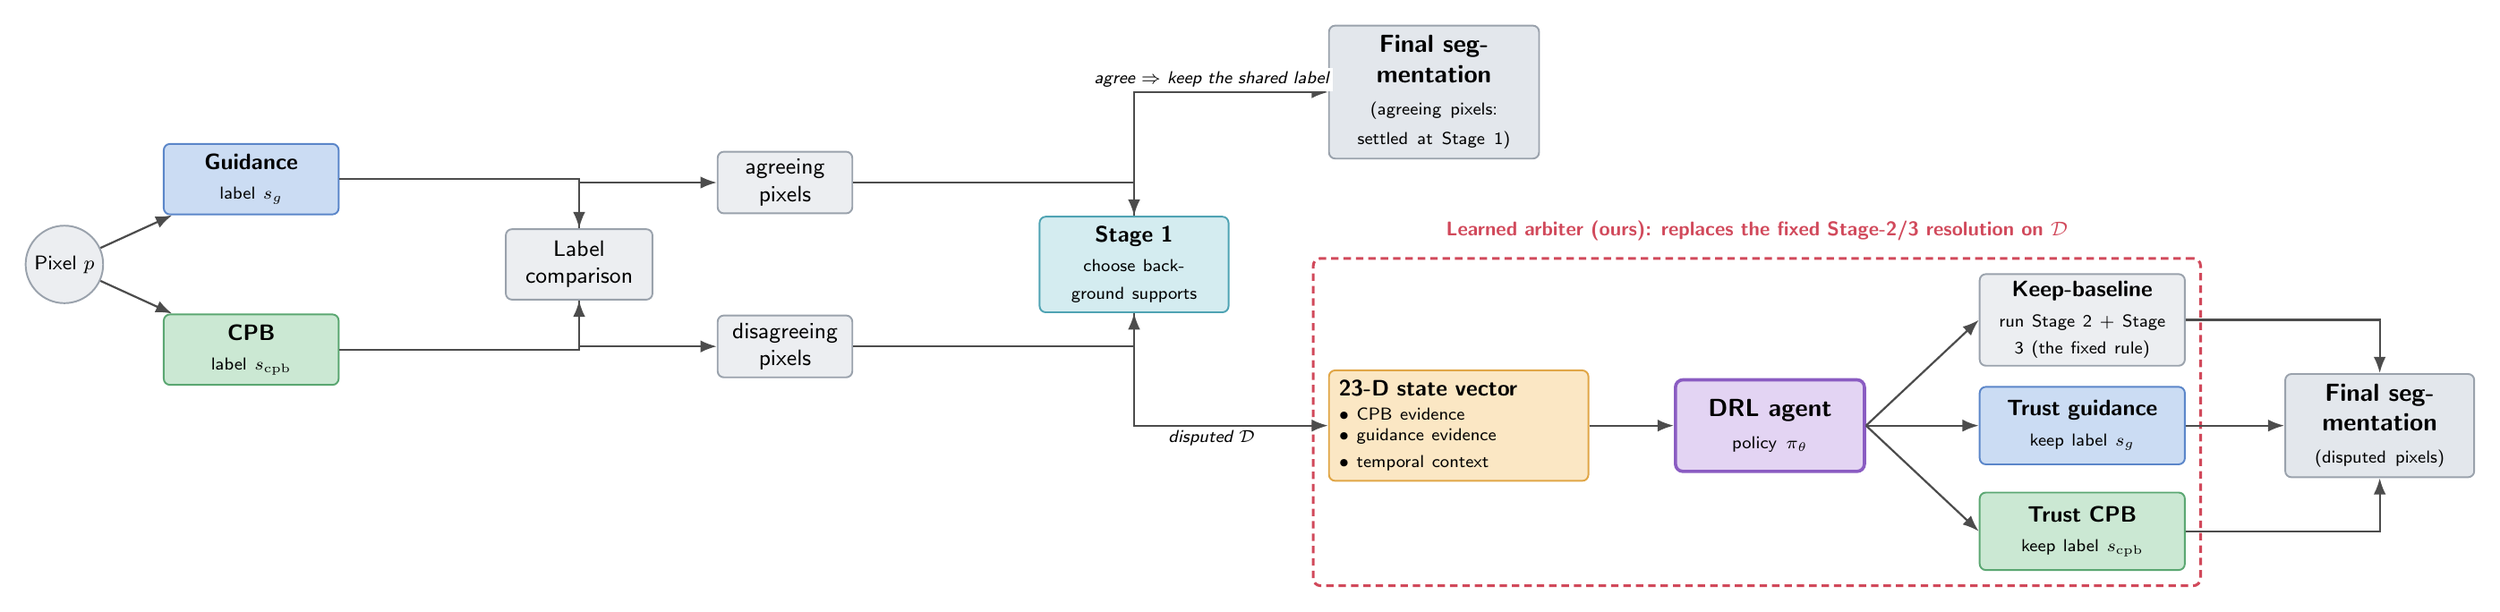
\begin{tikzpicture}[
  >=Latex, font=\sffamily\small, node distance=7mm, line width=0.7pt,
  box/.style   ={draw=cGrayL, rounded corners=2.5pt, align=center, minimum height=10mm,
                 inner sep=4pt, fill=cGray},
  guid/.style  ={box, fill=cBlue,  draw=cBlueL,  text width=22mm},
  cpb/.style   ={box, fill=cGreen, draw=cGreenL, text width=22mm},
  small/.style ={draw=cGrayL, rounded corners=2.5pt, align=center, fill=cGray,
                 inner sep=3pt, minimum height=8mm, text width=17mm},
  stage/.style ={draw=cStageL, rounded corners=2.5pt, align=center, fill=cStage,
                 inner sep=4pt, minimum height=12mm, text width=24mm},
  state/.style ={draw=cStateL, rounded corners=2.5pt, align=left, fill=cState,
                 inner sep=4pt, text width=34mm},
  agent/.style ={draw=cAgentL, rounded corners=3pt, align=center, fill=cAgent,
                 line width=1.3pt, inner sep=4pt, minimum height=13mm, text width=24mm,
                 font=\sffamily\bfseries},
  act/.style   ={draw=cGrayL, rounded corners=2.5pt, align=center, inner sep=3pt,
                 minimum height=11mm, text width=27mm},
  pix/.style   ={draw=cGrayL, circle, align=center, fill=cGray, inner sep=1pt,
                 minimum size=11mm, font=\sffamily\footnotesize},
  fin/.style   ={box, fill=cFin, draw=cGrayL, font=\sffamily\bfseries, text width=22mm},
  e/.style     ={->, thick, draw=black!70},
  lbl/.style   ={font=\sffamily\scriptsize\itshape, inner sep=1.5pt, fill=white}]

  %
  \node[pix] (pix) {Pixel $p$};
  \node[guid, above right=3mm and 10mm of pix] (guid) {\textbf{Guidance}\\[1pt]\scriptsize label $s_g$};
  \node[cpb, below right=3mm and 10mm of pix]  (cpb)  {\textbf{CPB}\\[1pt]\scriptsize label $s_{\mathrm{cpb}}$};
  \node[box, right=10mm of pix, text width=18mm] (cmp) at ($(guid)!0.5!(cpb)+(26mm,0)$) {Label\\comparison};
  \node[small, above right=2mm and 9mm of cmp] (agr) {agreeing\\pixels};
  \node[small, below right=2mm and 9mm of cmp] (dis) {disagreeing\\pixels};
  \node[stage, right=10mm of cmp] (s1) at ($(agr)!0.5!(dis)+(26mm,0)$)
       {\textbf{Stage 1}\\[1pt]\scriptsize choose background supports};

  \draw[e] (pix) -- (guid);
  \draw[e] (pix) -- (cpb);
  \draw[e] (guid) -| (cmp);
  \draw[e] (cpb)  -| (cmp);
  \draw[e] (cmp) |- (agr);
  \draw[e] (cmp) |- (dis);
  \draw[e] (agr) -| (s1);
  \draw[e] (dis) -| (s1);

  %
  \node[fin, above right=8mm and 14mm of s1, text width=27mm] (finA)
       {Final segmentation\\[1pt]\scriptsize\mdseries (agreeing pixels: settled at Stage 1)};
  \draw[e] (s1.north) |- node[lbl, pos=0.7, above]{agree $\Rightarrow$ keep the shared label} (finA.west);

  %
  \node[state, below right=8mm and 14mm of s1] (st)
       {\textbf{23-D state vector}\\[2pt]\scriptsize $\bullet$ CPB evidence\\$\bullet$ guidance evidence\\$\bullet$ temporal context};
  \draw[e] (s1.south) |- node[lbl, pos=0.7, below]{disputed $\mathcal{D}$} (st.west);

  \node[agent, right=12mm of st] (ag) {DRL agent\\[1pt]\scriptsize\mdseries policy $\pi_\theta$};
  \draw[e] (st) -- (ag);

  \node[act, fill=cGray,  draw=cGrayL,  right=16mm of ag, yshift=15mm]  (a0) {\textbf{Keep-baseline}\\[1pt]\scriptsize run Stage 2 $+$ Stage 3 (the fixed rule)};
  \node[act, fill=cBlue,  draw=cBlueL,  right=16mm of ag, yshift=0mm]   (a1) {\textbf{Trust guidance}\\[1pt]\scriptsize keep label $s_g$};
  \node[act, fill=cGreen, draw=cGreenL, right=16mm of ag, yshift=-15mm] (a2) {\textbf{Trust CPB}\\[1pt]\scriptsize keep label $s_{\mathrm{cpb}}$};
  \draw[e] (ag.east) -- (a0.west);
  \draw[e] (ag.east) -- (a1.west);
  \draw[e] (ag.east) -- (a2.west);

  \node[fin, right=14mm of a1, text width=24mm] (finD)
       {Final segmentation\\[1pt]\scriptsize\mdseries (disputed pixels)};
  \draw[e] (a0.east) -| (finD.north);
  \draw[e] (a1.east) -- (finD.west);
  \draw[e] (a2.east) -| (finD.south);

  % dashed box: learned part
  \begin{scope}[on background layer]
    \node[draw=cAccent, densely dashed, line width=1.1pt, rounded corners=3pt,
          fit=(st)(ag)(a0)(a2), inner sep=6pt] (learn) {};
  \end{scope}
  \node[font=\sffamily\footnotesize\bfseries, cAccent, above=1mm of learn]
       {Learned arbiter (ours): replaces the fixed Stage-2/3 resolution on $\mathcal{D}$};
\end{tikzpicture}
\end{document}
